% Figure 4 of "The architecture of blockchain value: capabilities, pillars, and growth dynamics"
% (Papadogiannis, 2026, Front. Blockchain 9:1747512). Drawing code as in the author's manuscript.
% Compile with: pdflatex fig4_capability_sets.tex
\documentclass[border=6pt]{standalone}
\usepackage{amsmath, amssymb}
\usepackage{tikz}
\usetikzlibrary{positioning, shapes, arrows.meta, calc, backgrounds}
\begin{document}
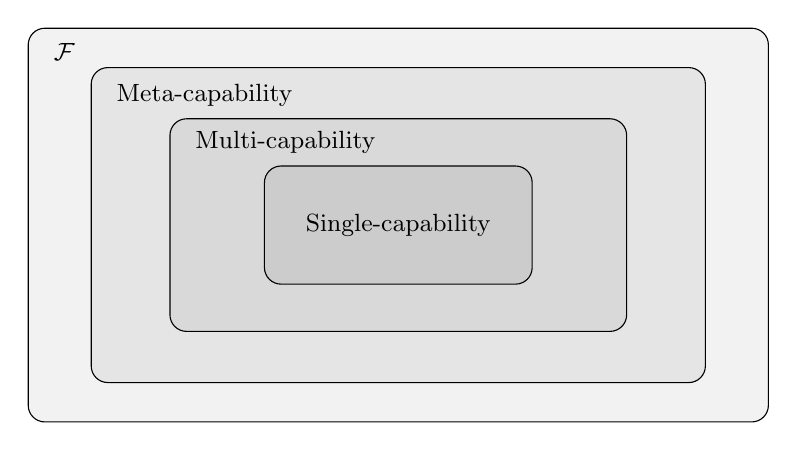
\begin{tikzpicture}[font=\small]
  % Outer set F
  \fill[gray!10, draw=black, rounded corners=6pt] (-4.7,-2.5) rectangle (4.7,2.5);
  \node[anchor=west] at (-4.5,2.2) {$\mathcal{F}$};

  % Meta-capability
  \fill[gray!20, draw=black, rounded corners=6pt] (-3.9,-2.0) rectangle (3.9,2.0);
  \node[anchor=west] at (-3.7,1.65) {Meta-capability};

  % Multi-capability
  \fill[gray!30, draw=black, rounded corners=6pt] (-2.9,-1.35) rectangle (2.9,1.35);
  \node[anchor=west] at (-2.7,1.05) {Multi-capability};

  % Single-capability
  \fill[gray!40, draw=black, rounded corners=6pt] (-1.7,-0.75) rectangle (1.7,0.75);
  \node[text width=3.1cm, align=center] at (0,0) {Single-capability};
\end{tikzpicture}
\end{document}
